\section{Rezultatai}

\subsection{Difuzijos įtaka}


\subsection{Kinetikų soties vertė}
\label{page:saturation}
\begin{figure}[h]
  \centering
	\subfloat[Logaritminė skalė]{
		\label{fig:saturation_log}
		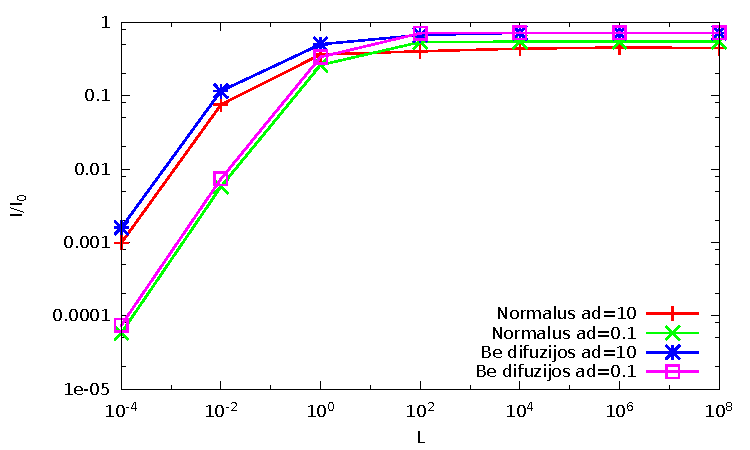
\includegraphics[width=0.5\textwidth]{./media/pdf/saturation.pdf}
		}
	\subfloat[Pusiau logaritminė skalė]{
		\label{fig:saturation_semilog}
		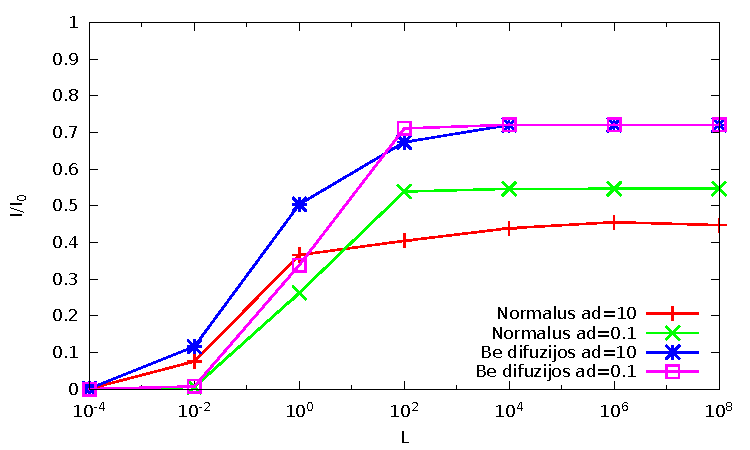
\includegraphics[width=0.5\textwidth]{./media/pdf/semilogsaturation.pdf}
		}
  \caption{Kinetikų maksimumo vertės sotinimas nuo šviesos intensyvumo, priklausomai nuo difuzijos ir sugerties profilio, esant minimaliam užlaikymui $t_{delay}$}
  \label{fig:saturation}
\end{figure}

Rekombinacijos įvertinimui naudojama srovės soties vertė, kai nėra užlaikymo laiko tarp šviesos impulso ir ištraukiančios įtampos impulso. Atlikę srovės soties skaičiavimus (žr. \ref{fig:saturation} pav.) pastebime, jog soties vertė, neįskaitant difuzijos, dėl užlaikymo laiko pakinta per pastovų dydį, nepriklausomai nuo sugerties profilio $\alpha d$. Įskaičius difuziją, srovės soties vertė ima priklausyti nuo $\alpha d$.

Iš šių rezultatų seka dvi išvados:
\begin{itemize}
\item Rekombinacijos įvertinimas pagal soties reiškinį jautrus užlaikymo laikui $t_{delay}$.
\item Veikiant difuzijai kinetikų soties vertė priklauso nuo krūvininkų sugerties profilio.
\end{itemize}

\subsection{Rekombinacijos koeficiento vertė}

\begin{figure}
  \centering
	\subfloat[Be difuzijos]{
		\label{fig:delays_nodiff}
		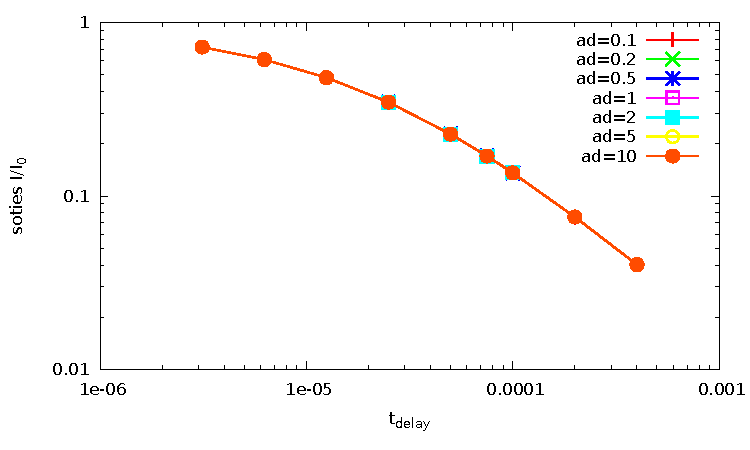
\includegraphics[width=0.5\textwidth]{./media/pdf/delays_nodiff.pdf}
		}
	\subfloat[Su difuzija]{
		\label{fig:delays_diff}
		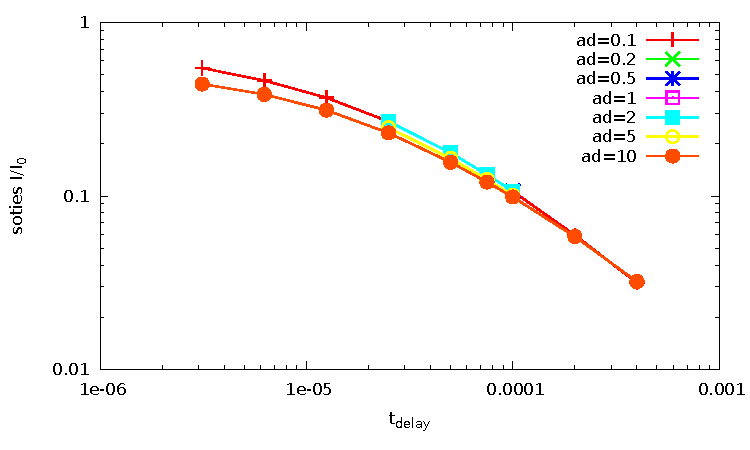
\includegraphics[width=0.5\textwidth]{./media/pdf/delays_diff.pdf}
		}
  \caption{Photo-CELIV srovės kinetikų soties vertės priklausomybės nuo užlaikymo trukmės $t_{delay}$}
  \label{fig:delays}
\end{figure}

Norėdami atmesti užlaikymo laiko įtaką kinetikos soties srovei atlikome skaičiavimus su skirtingomis užlaikymo trukmėmis, kurių rezultatai pavaizduoti \ref{fig:delays} paveiksliuke.

Pastebime, [kažkokį rezultatą]

Šie rezultatai dar kartą parodo, jog veikiant difuzijai kinetikų soties vertė priklauso nuo krūvininkų sugerties profilio.

\subsection{Judrio vertės matavimai}
Pagal šią formulę skaičiuojant krūvininkų judrį iš įsisotinusių srovės kinetikų maksimumų gaunama krūvinikų judrio priklausomybė nuo užlaikymo laiko pavaizduota \ref{fig:mobility} paveiksliuke. Anksčiau panašūs rezultatai buvo aiškinami krūvininkų prilipimu \cite{•}. Tačiau šioje simuliacijoje krūvininkų prilipimas nėra įskaitomas, taigi egzistuoja kitos priežastys šiam kitimui.

\begin{figure}
  \centering
	\subfloat[Be difuzijos]{
		\label{fig:mobility_nodiff}
		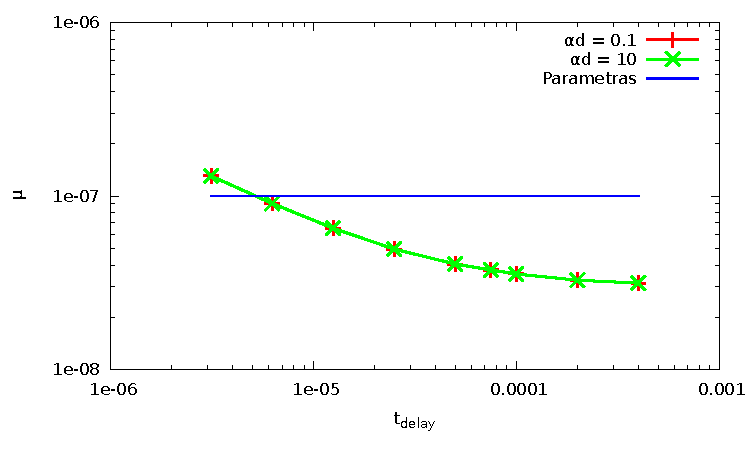
\includegraphics[width=0.5\textwidth]{./media/pdf/log_mobility_nodiff.pdf}
		}
	\subfloat[Su difuzija]{
		\label{fig:mobility_diff}
		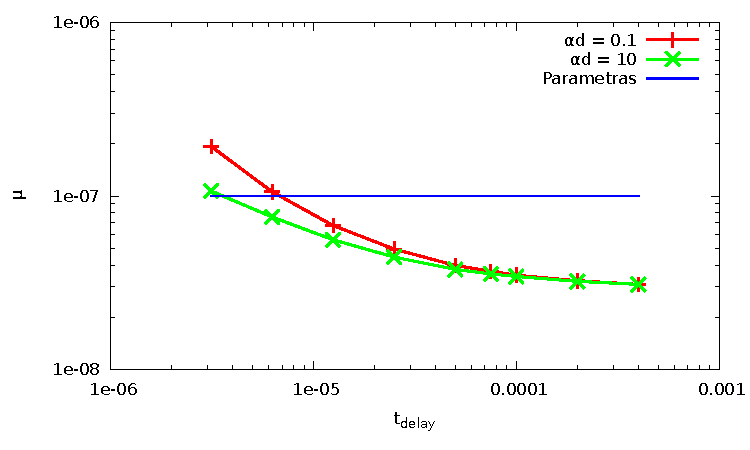
\includegraphics[width=0.5\textwidth]{./media/pdf/log_mobility_diff.pdf}
		}
  \caption{Krūvininkų judrio skaičiavimo pagal \eqref{eq:judris} formulę rezultatų priklausomybė nuo $t_{delay}$}
  \label{fig:mobility}
\end{figure}

